\chapter{Comparative Analysis}
The evaluation of the proposed model occurs in three phases. In the first phase, the model is tested for its ability to predict emotions across different target domains, such as books, music, movies, and games, along with statistical analysis. Two models are trained on the GoEmotions dataset, PRADO and BERT, namely FL-PRADO and FL-BERT, using the experimental setup in Section 3.3. The second phase of evaluation compares these two models exclusively on different datasets. In addition, two versions of FL-PRADO cross-domain recommendation are implemented, V1 and V2, as described in Section 3.4. The comparison among these two versions and BERT is performed on various metrics. The third phase of evaluation compares the proposed model with baseline recommenders and their FL frameworks.

\section{Evaluation metrics}
The evaluation metrics used to assess the proposed model’s performance are discussed in this section.

\subsection{Over queries and target domain size:}
\begin{equation}
  \text{HR@K} = \frac{1}{Q} \sum_{q} \mathbf{1}\left[ r_{q} \leq K \right]
  \label{eq:ch5_4_21}
\end{equation}
\begin{equation}
  \text{NDCG@K} = \frac{1}{Q} \sum_{q} \frac{\mathbf{1}\left[ r_{q} \leq K \right]}{\log_{2}(r_{q} + 1)}
  \label{eq:ch5_4_22}
\end{equation}
\begin{equation}
  \text{MRR} = \frac{1}{Q} \sum_{q} \frac{1}{r_{q}}
  \label{eq:ch5_4_23}
\end{equation}
\begin{equation}
  \mathbb{E}[\text{HR@K}] = \frac{K}{N}, \quad \mathbb{E}[\text{NDCG@K}] = \frac{1}{N} \sum_{j=1}^{K} \frac{1}{\log_{2}(j+1)}, \quad \mathbb{E}[\text{MRR}] = \frac{H_{N}}{N}, \quad \text{median} = \frac{N+1}{2}
  \label{eq:ch5_4_24}
\end{equation}

\section{Recommendation model evaluation}
The FL-PRADO model is tested for its ability to predict emotions across different target domains, such as books, music, movies, and games, along with statistical analysis. Two models are trained on the GoEmotions dataset, PRADO and BERT, namely FL-PRADO and FL-BERT, using the experimental setup in Section 3.3. The second phase of evaluation compares these two models exclusively on different datasets. Along with this, two versions of FL-PRADO are implemented V1 and V2 as per description in Section 3.4. The comparison among these two versions and BERT is performed on various metrics.  The third phase of evaluation compares the proposed model with baseline recommenders and their FL frameworks.

The datasets used for comparative analysis are described in Table 5.1. It also contains details regarding total number of items in the dataset and chunks created for those items. The Items in Table 5.1 indicate the total number of unique reviews in the respective dataset. The chunks are small text segments created after splitting each item into shorter parts. The number under the hunks column indicates, for the given data, how many segments are created. The chunking column indicates the process applied for creating these chunks for different datasets.

\setlength{\tabcolsep}{4pt}
{\footnotesize
\begin{longtable}{|p{1.8cm}|p{3cm}|p{1.5cm}|p{1.5cm}|p{3cm}|}
\caption{Dataset Statistics and Text Chunking Strategy}
\label{tab:ch5_t1} \\
\hline
Domain & Source & Items & Chunks & \makecell{Chunking \\ Strategy} \\
\hline
\endfirsthead
\hline
Domain & Source & Items & Chunks & \makecell{Chunking \\ Strategy} \\
\hline
\endhead
\hline
\endfoot
\makecell{Books \\ (orig.)} \cite{ref81} & \makecell{Amazon reviews \\ (unique\_reviews)} & 9,970 & 10,000 & \makecell{one review \\ per title} \\
\hline
Books A \cite{ref93} & \makecell{same, titles \\ $\geq 2$ reviews} & 2,197 & 4,962 & whole reviews \\
\hline
Books B \cite{ref94} & \makecell{Goodreads-100k \\ descriptions} & 12,000 & 92,622 & \makecell{sentences \\ ($\leq 20$)} \\
\hline
Movies \cite{ref95} & \makecell{CMU Movie \\ Summary Corpus} & 12,000 & 255,602 & \makecell{plot sentences \\ ($\leq 40$)} \\
\hline
Music \cite{ref96} & \makecell{Genius lyrics \\ (5 genre tags)} & 10,398 & 141,633 & \makecell{4-line stanzas \\ ($\leq 30$)} \\
\hline
Games \cite{ref97} & \makecell{Steam catalog \\ top titles} & 11,968 & 187,738 & \makecell{store-page sent. \\ ($\leq 30$)} \\
\hline
\end{longtable}
\setlength{\tabcolsep}{6pt}
} % end footnotesize

\subsection{Performance Evaluation across Domains}
In this phase, FL-PRADO(V2) is tested for its ability to predict emotions across different target domains, such as books, music, movies, and games. The proposed system uses 128-dimensional federated embeddings to represent documents, a fully federated PRADO model with 120-client MLServer FedAvg, and a leak-free split-half protocol to prevent data leakage during evaluation.

\setlength{\tabcolsep}{4pt}
{\footnotesize
\begin{longtable}{|p{1.5cm}|p{1.4cm}|p{1.4cm}|p{1.4cm}|p{1.4cm}|p{1.8cm}|p{1.4cm}|}
\caption{Ranking Performance of the Proposed CDR Framework Across Target Domains}
\label{tab:ch5_t2} \\
\hline
\makecell{Target \\ Domain} & \makecell{HR@10 \\ (\%)} & \makecell{HR@10 \\ over Rand.} & \makecell{NDCG@10 \\ (\%)} & \makecell{MRR \\ (\%)} & \makecell{median rank \\ (domain size)} & \makecell{Random \\ med.\ Rank} \\
\hline
\endfirsthead
\hline
\makecell{Target \\ Domain} & \makecell{HR@10 \\ (\%)} & \makecell{HR@10 \\ over Rand.} & \makecell{NDCG@10 \\ (\%)} & \makecell{MRR \\ (\%)} & \makecell{median rank \\ (domain size)} & \makecell{Random \\ med.\ Rank} \\
\hline
\endhead
\hline
\endfoot
Movies & 27.4 & $329\times$ & 20.9 & 19.5 & 272 of 12,000 & 6,000 \\
\hline
Music & 79.6 & $828\times$ & 75.7 & 74.7 & 1 of 10,398 & 5,200 \\
\hline
Games & 12.0 & $143\times$ & 8.02 & 7.26 & 1,268 of 11,968 & 5,984 \\
\hline
Books & 6.27 & $75\times$ & 4.02 & 3.70 & 2,192 of 12,000 & 6,000 \\
\hline
\end{longtable}
\setlength{\tabcolsep}{6pt}
} % end footnotesize

A leak-free split-half protocol ensures that only one half of an item’s text is used. The other half is used to build the item’s emotion profile. Consider an example: a music query contains 6 lyric stanzas, and a movie query consists of 12 plot sentences. This split-half protocol ensures that the indexed representation and the query never share the same content. This prevents information leakage and makes evaluation more realistic. The performance of the proposed model is best for Music, good for Movies, but Games and Books are challenging domains.

The median rank in Table 5.2 indicates the position of the correct item in the ranking list. The music domain has a median rank of 1. It means that for at least half of the different music queries, the correct song is ranked first from the 10,398 candidates. In contrast, the random recommender described in Eq. 4.24 would rank the correct item at 5200th position. The probability (HR@10) that the correct item appears in the top 10 is presented in the graph (Figure 5.2.X).

\begin{figure}[htbp]
  \centering
  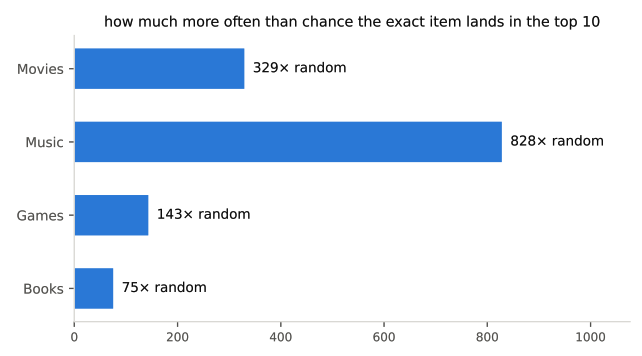
\includegraphics[width=0.8\textwidth]{figures/image32}
  \caption{HR@10 performance of FL-PRADO over different target domains.}
  \label{fig:ch5_f1}
\end{figure}

Figure 5.2 shows the cumulative distribution of the true item’s rank. The x-axis is a log-scale representation of the rank assigned to the correct item among different items in the candidate set. The Y-axis shows the cumulative percentage of queries for which the correct item appears at/ above rank. The steeper rising curve of FL-PRADO indicates that the correct item is consistently ranked near the top. The dashed gray curve shows the random recommender performance.

\begin{figure}[htbp]
  \centering
  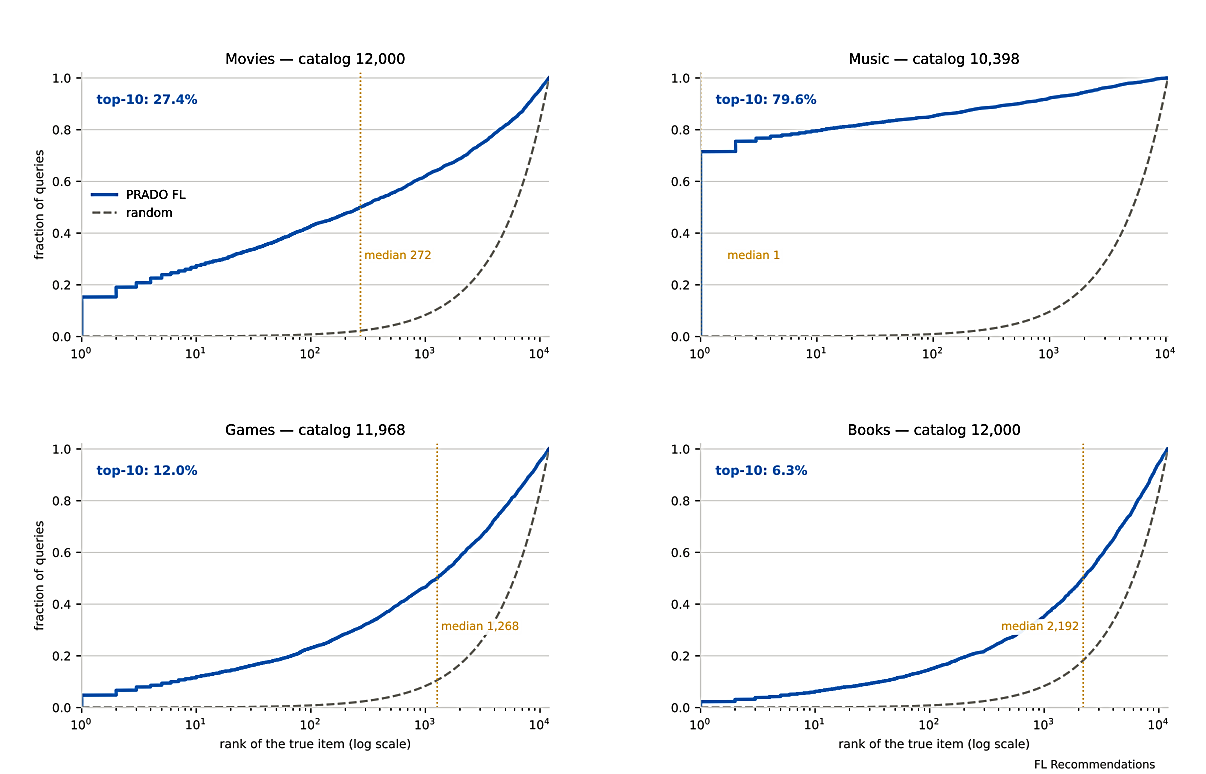
\includegraphics[width=0.8\textwidth]{figures/image33}
  \caption{Cumulative distribution of the true item's rank.}
  \label{fig:ch5_f2}
\end{figure}

\subsection{FL-PRADO (V1 vs. V2)}
Section 4.3 describes the two different implementations of FL-PRADO as V1 and V2 (embeddings + document queries, same MLServer FedAvg weights $\cdot$ 128-d penultimate embedding $\cdot$ query = held-out half of the item's chunks $\cdot$ 3-view ensemble scorer). This section describes the performance difference between these two versions. Table 5.3 demonstrates the enhanced retrieval pipeline (V2) results. V1 and V2 receive the same federated model weights. HR@10 measures the percentage of those queries for which the correct item is listed among the top 10 retrieved results. Out of four target domains, for Movies, V2 achieves a 27.4\% hit ratio, which is a 74X improvement over V1 and a 23X improvement over BERT. This indicates V2 captures movie semantics much more effectively. For music, it receives the highest hit ratio. For Games and Books, the HR@10 is lower, but there is still improvement over V1 and BERT. Median Rank indicates the position of the correct item in the ranking list, lower values are better. From Table 5.3, median rank improves for Movies in V2 drastically as compared to V1 and BERT. For music, it is 1. This indicates the correct song is top-ranked for more than half of all the queries. There is substantial improvement in Median rank for the Games and Books domains too.

Mean Reciprocal Rank (MRR) gives the average of the reciprocal of its rank. Larger values indicate better ranking. For all four domains, there is improvement in MRR (> 75X on average).

\begin{table}[htbp]
  \centering
  \caption{Headline Retrieval Results}
  \label{tab:ch5_t3}
  \begin{tabular}{|c|c|c|c|c|c|c|c|}
    \hline
    & \multicolumn{4}{c|}{HR@10} & \multicolumn{3}{c|}{Median Rank} \\
    \cline{2-8}
    Domain & v2 & v1 & BERT & Random & v2 & v1 & Random \\
    \hline
    Movies & 27.4\% & 0.37\% & 1.17\% & 0.083\% & 272 & 4,376 & 6,000 \\
    \hline
    Music & 79.6\% & 11.90\% & 6.10\% & 0.096\% & 1 & 1,204 & 5,200 \\
    \hline
    Games & 12.0\% & 0.37\% & 0.67\% & 0.084\% & 1,268 & 4,244 & 5,984 \\
    \hline
    Books B & 6.3\% & 0.57\% & 2.20\% & 0.083\% & 2,192 & 4,600 & 6,000 \\
    \hline
    & \multicolumn{4}{c|}{MRR} & \multicolumn{3}{c|}{NDCG@10} \\
    \cline{2-8}
    Domain & v2 & v1 & BERT & Random & v2 & v1 & BERT \\
    \hline
    Movies & 19.5\% & 0.23\% & 0.57\% & 0.083\% & 20.9\% & 0.17\% & 0.56\% \\
    \hline
    Music & 74.7\% & 8.12\% & 3.33\% & 0.095\% & 75.7\% & 8.68\% & 3.62\% \\
    \hline
    Games & 7.3\% & 0.23\% & 0.38\% & 0.083\% & 8.0\% & 0.17\% & 0.29\% \\
    \hline
    Books B & 3.7\% & 0.40\% & 1.11\% & 0.083\% & 4.0\% & 0.34\% & 1.10\% \\
    \hline
  \end{tabular}
\end{table}

NDCG@10 (Normalized Discounted Cumulative Gain) rewards correct items appearing at the

top 10 results. For Movies, V2 achieves 20.9\%, which is substantially greater than V1 and BERT.

For Music, it is highest and lower for Games and Books.

\begin{figure}[htbp]
  \centering
  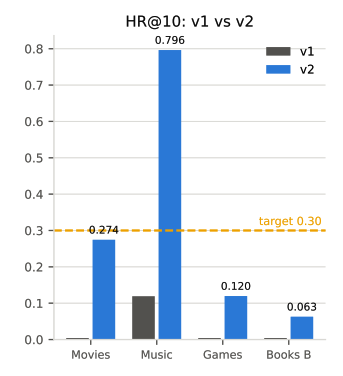
\includegraphics[width=0.8\textwidth]{figures/image34}
  \caption{Hit rate comparison between V1 and V2}
  \label{fig:ch5_f3}
\end{figure}

Figure  5.3 demonstrated the Hit rate comparison between two versions of the proposed model.

\subsection{CDR Frameworks Evaluation}
In the field of cross-domain recommendation (CDR), researchers have explored a number of representative models, each using a different learning paradigm to transfer knowledge across domains. Since there aren't any directly comparable baseline approaches, we selected four popular and typical models: EMCDR \cite{ref86}, CDFLM \cite{ref87}, ANR \cite{ref88}, and MFPCDR \cite{ref89}.

The EMCDR framework uses a multilayer perceptron (MLP) to learn how to translate nonlinearly between the source and target domains. This helps improve cross-domain recommendation effectiveness by aligning user and item embeddings. The ANR model, in contrast, employs an attention-based process within an aspect-oriented framework. The model is first trained on the target domain. Then, reviews from the source domain that are related to the target domain are added to improve the accuracy of the recommendations \cite{ref87} .

The CDLFM approach employs latent feature mapping to find patterns of user behavior in various fields. It employs a domain-based gradient boosting tree to transfer knowledge across domains to aid the cold-start problem by using some hidden user attributes \cite{ref88}.

The MFPCDR framework builds on this concept in a federated learning environment, integrating meta-learning and attention techniques to provide customized recommendations while preserving privacy \cite{ref89}.

To enable a comprehensive comparison between these methods, it is evident that they differ significantly in application aspects, privacy principles, and design procedures. The EMCDR model does not have any privacy-saving mechanism that cuts across the Books and Movies spheres. It applies a multilayer perceptron. The Books and Movies domains also apply to CDLFM, which maps latent features with a gradient boosting tree, but it is not privacy-preserving. The ANR model is applicable to both the Movies and CDs domains and has an attention mechanism, which enhances recommendation quality. It, however, does not consider privacy. MFPCDR, conversely, incorporates attention and transfer learning into a federated learning system, thus protecting user privacy in the Books and Movies fields.  The MFCDR with the PRADO(FL-PRADO) model builds on these ideas by combining a projected attention network with transfer learning to enable privacy-preserving knowledge transfer between the Emotion and different domains (Books, Movies, Music, and Games). This makes it a more secure and flexible way to recommend things across domains.

The original centralized EMCDR, ANR, and CDFLM models were adapted into the federated learning environment. By comparing all models under the federated settings, we ensure a fair and consistent comparison between different models, which eliminates bias caused by different training architectures.

Dataset across CDR: Different source domains across the same target domain are used for comparative analysis to strengthen the concept of emotion as a base for personalized recommendation.

The comparison is performed across the following source-domain to target-domain pairs: EMCDR (Books, Movies), ANR (Music, Movies), CDFLM (Ratings, Movies), MFPCDR (Books, Movies), and FL-PRADO (Emotions, Movies).

The models tested and shown in Table 5.4 are ranked in terms of HR@10, HR@20, NDCG@10, NDCG@20, and MRR.

Table 5.4 and the plot in Figure 5.4 benchmark the recommendation performance of the proposed FL-PRADO model against the best baseline models. FL-PRADO achieves the highest HR@10 of 27.4\%, outperforming MFPCDR (17.21\%) by 10.19 percentage points (59.2\%) and FL-EMCDR (15.35\%) by 12.05 percentage points (78.5\%). Similarly, FL-PRADO attains the best HR@20 of 31.6\%, exceeding MFPCDR (21.35\%) by 10.25 percentage points (48.0\%) and FL-EMCDR (21.61\%) by 9.99 percentage points (46.2\%).

\begin{longtable}{|p{2.5cm}|p{2cm}|p{2cm}|p{2cm}|p{2cm}|p{2cm}|}
\caption{Analysis of Ranking Quality for different models}
\label{tab:ch5_t4} \\
\hline
Model & HR@10 & HR@20 & NDCG@10 & NDCG@20 & MRR \\
\hline
\endfirsthead
\hline
Model & HR@10 & HR@20 & NDCG@10 & NDCG@20 & MRR \\
\hline
\endhead
\hline
\endfoot
EMCDR* & 9.10\% & 14.46\% & 4.97\% & 6.32\% & 4.19\% \\
\hline
ANR* & 4.54\% & 6.87\% & 3.65\% & 5.97\% & 3.91\% \\
\hline
CDFLM* & 8.94\% & 17.42\% & 5.44\% & 6.18\% & 4.22\% \\
\hline
FL-EMCDR & 15.35\% & 21.61\% & 9.73\% & 12.05\% & 8.47\% \\
\hline
FL-ANR & 7.31\% & 12.96\% & 6.39\% & 9.80\% & 6.51\% \\
\hline
FL-CDFLM & 7.72\% & 13.04\% & 3.37\% & 4.71\% & 3.18\% \\
\hline
MFPCDR & 17.21\% & 21.35\% & 12.33\% & 13.14\% & 10.13\% \\
\hline
FL-PRADO & 27.4\% & 31.6\% & 20.9\% & 21.8\% & 19.5\% \\
\hline
\multicolumn{6}{|l|}{* Indicates a non-FL environment for the model training} \\
\hline
\end{longtable}

\begin{figure}[htbp]
  \centering
  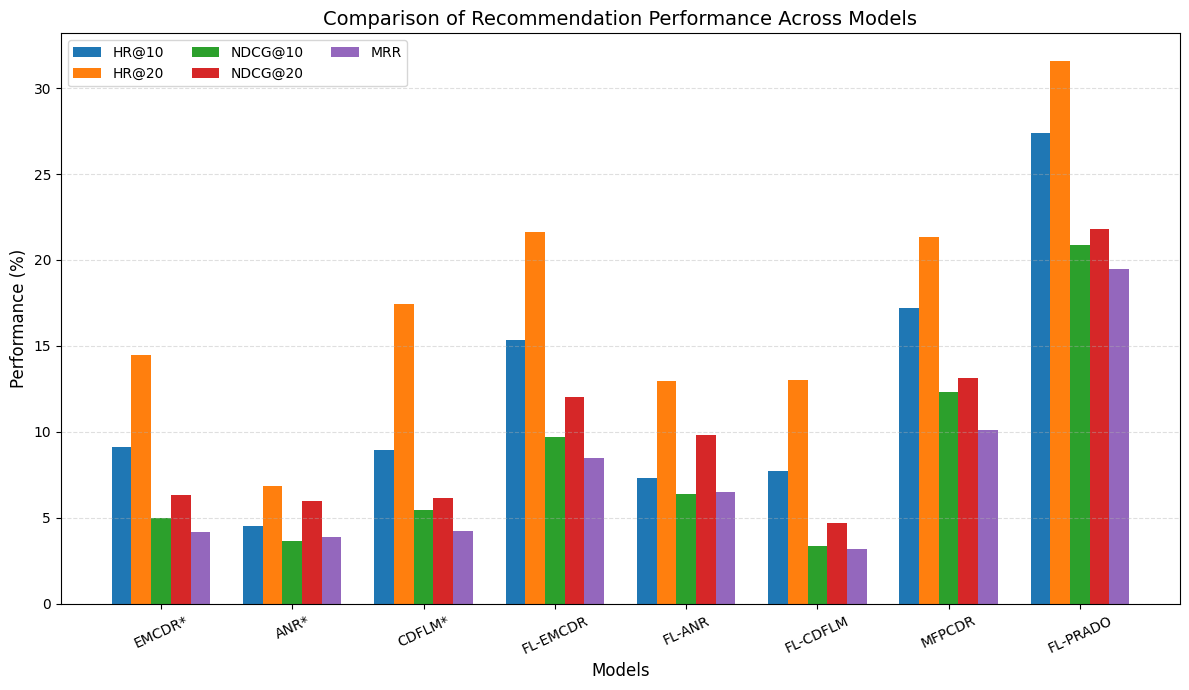
\includegraphics[width=0.8\textwidth]{figures/image35}
  \caption{Recommendation Performance Comparison}
  \label{fig:ch5_f4}
\end{figure}

The NDCG@10 of FL-PRADO is 20.9\%, an improvement of 69.5\% over MFPCDR (12.33\%) and 114.8\% over FL-EMCDR (9.73\%). Likewise, NDCG@20 reaches 21.8\%, surpassing MFPCDR (13.14\%) by 65.9\% and FL-EMCDR (12.05\%) by 80.9\%.

In terms of MRR, FL-PRADO achieves 19.5\%, improving upon MFPCDR (10.13\%) by 92.5\% and FL-EMCDR (8.47\%) by 130.2\%. The results show that FL-PRADO achieves the best retrieval accuracy and ranking performance compared to other state-of-the-art non-federated and federated recommendation models.

In general, the experimental results confirm that the FL-PRADO(V2) model gives the best top-K recommendations and the best ranking quality among all the models evaluated. The steady increase in HR, NDCG, and MRR scores confirms the success of incorporating federated representation learning based on PRADO with the proposed cross-domain recommendation framework for preserving privacy while also achieving better recommendation performance.

\section{Summary}
This chapter conducted a detailed review of the proposed MFCDR concept across various recommendation areas. The proposed FL-PRADO model achieved the best performance in terms of HR@10, HR@20, NDCG, and MRR. The highest Hit Rate (HR@10) of the proposed model, i.e., 79.6\%, is recorded for song recommendation (Music), along with MRR 74.7\%, median rank 1, and NDGC@10 is 75.7. Comparative experiments shown in Figure 5.4 demonstrate that the proposed FL-PRADO model consistently outperformed the centralized, federated, and state-of-the-art recommendation models. The results demonstrate the effectiveness of federated learning combined with PRADO in providing privacy-preserving cross-domain recommendations, with higher recommendation accuracy, better ranking quality, scalability, and user privacy. This chapter meets Objective 4.

